% Forløbig resultater
% Opsætning
% Fuel
% Afstand
% Fremtidige tests/arbejde
% Konklusion


\section{Evaluation}
\begin{frame}{Test Setup}



\begin{columns}
	\begin{column}{0.7\textwidth}
		\begin{itemize}
		\item SUMO- Simulation of Urban MObility\\
		\item Real world road network\\
		\item Real world Traffic light phases\\
		\item Real world OD matrix\\
		\end{itemize}
	\end{column}

	\begin{column}{0.3\textwidth}
		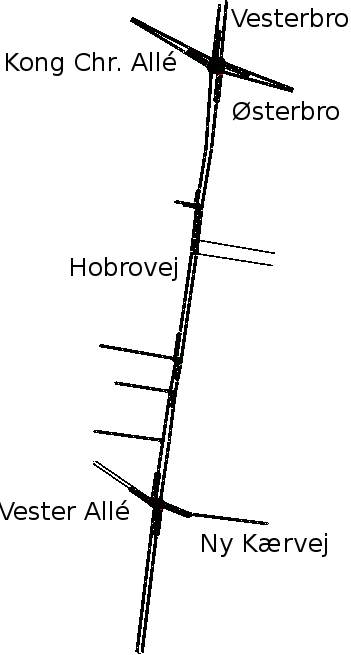
\includegraphics[width=0.8\textwidth]{images/Hobrovej.png}
	\end{column}
\end{columns}
\end{frame}

\begin{frame}{SUMO presentation}
\end{frame}

\begin{frame}{Fuelsaving}
	\begin{figure}
	\begin{tikzpicture}[scale=0.6]
	\begin{axis}[xlabel=Routes,xticklabel=\empty,ylabel=Fuel consumption,bar width=1pt,]
	\addplot[ybar, blue] table[x=Route,y=Fuel] {TestResults/0/avg.dat};
	\addplot[ybar, red] table[x=Route,y=Fuel] {TestResults/100/avg.dat};
	\draw[thick, red] (axis cs:0,138) -- (axis cs:109,138);
	\draw[thick, blue] (axis cs:0,162) -- (axis cs:109,162);
	\end{axis}
	\end{tikzpicture}
	\caption{Average fuel consumption with (red) and without \tech (blue)}\label{tik:fuel:avg}
	\end{figure}
\end{frame}


\begin{frame}{Distance}



\begin{columns}
	\begin{figure}[htb]
	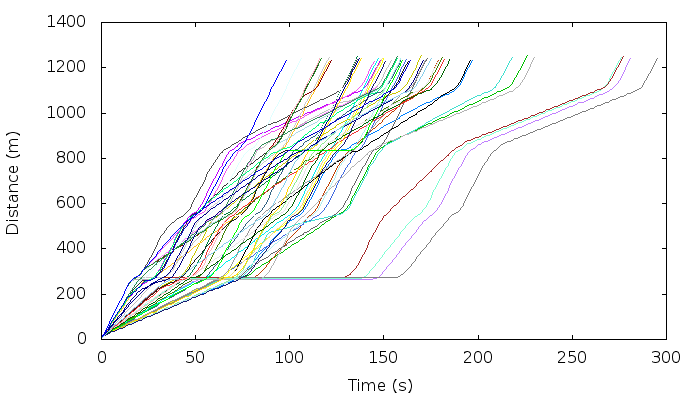
\includegraphics[width=0.5\textwidth]{images/tp0/distance100.png}
	\caption{Speed graph}
	\label{fig:TestResults:distance100}
	\end{figure}

	\begin{column}{0.5\textwidth}
	
\begin{figure}
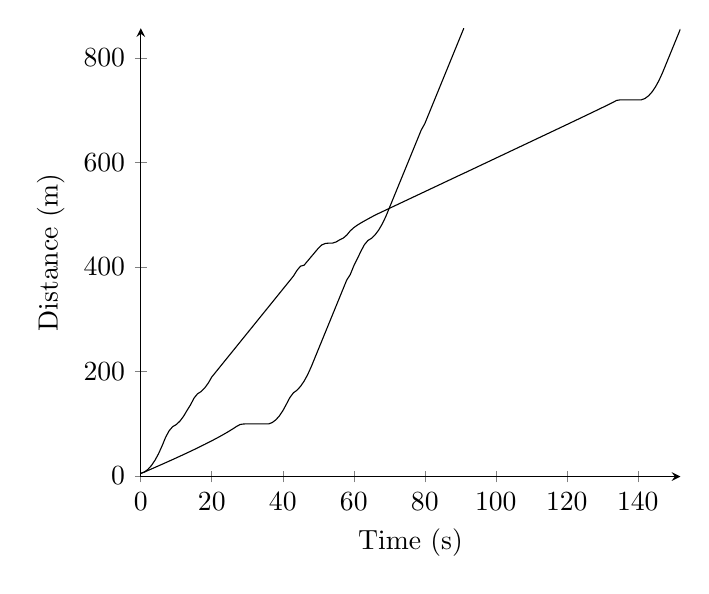
\begin{tikzpicture}
\begin{axis}[
legend style={anchor=west},
axis x line=bottom,
axis y line=left,
ymin=-1,
xlabel=Time (s),
ylabel=Distance (m),
]
\addplot[] coordinates {
(0, 5.1)
(1, 7.6)
(2, 10.551264739)
(3, 13.5148458518)
(4, 16.491720024)
(5, 19.4829705626)
(6, 22.4898024406)
(7, 25.5135599774)
(8, 28.555747716)
(9, 31.6180551961)
(10, 34.7023865031)
(11, 37.810895714)
(12, 40.9460296665)
(13, 44.1105798987)
(14, 47.3077461535)
(15, 50.5412145976)
(16, 53.8152549271)
(17, 57.1348419561)
(18, 60.5058092771)
(19, 63.9350454196)
(20, 67.4307470306)
(21, 71.0027496137)
(22, 74.6629653545)
(23, 78.4259712621)
(24, 82.309812202)
(25, 86.3371174595)
(26, 90.5366852977)
(27, 94.9457842613)
(28, 98.6044896023)
(29, 99.6320158223)
(30, 99.7193641886)
(31, 99.7193641886)
(32, 99.7193641886)
(33, 99.7193641886)
(34, 99.7193641886)
(35, 99.7193641886)
(36, 99.7193641886)
(37, 102.219364189)
(38, 107.219364189)
(39, 114.719364189)
(40, 124.719364189)
(41, 137.219364189)
(42, 150.125095958)
(43, 159.234657451)
(44, 164.142641251)
(45, 171.550625052)
(46, 181.458608852)
(47, 193.866592652)
(48, 208.774576453)
(49, 225.374576453)
(50, 241.974576453)
(51, 258.574576453)
(52, 275.174576453)
(53, 291.774576453)
(54, 308.374576453)
(55, 324.974576453)
(56, 341.574576453)
(57, 358.174576453)
(58, 374.774576453)
(59, 385.384576453)
(60, 401.984576453)
(61, 415.584576453)
(62, 429.92347141)
(63, 442.651450477)
(64, 450.734866052)
(65, 454.801722929)
(66, 461.368579805)
(67, 470.435436682)
(68, 482.002293558)
(69, 496.069150435)
(70, 512.636007311)
(71, 529.236007311)
(72, 545.836007311)
(73, 562.436007311)
(74, 578.936007311)
(75, 595.536007311)
(76, 612.136007311)
(77, 628.736007311)
(78, 645.336007311)
(79, 661.936007311)
(80, 674.076007311)
(81, 690.676007311)
(82, 707.276007311)
(83, 723.876007311)
(84, 740.476007311)
(85, 757.076007311)
(86, 773.676007311)
(87, 790.276007311)
(88, 806.876007311)
(89, 823.476007311)
(90, 840.076007311)
(91, 856.676007311)
};
\addplot[] coordinates {
(0, 5.1)
(1, 7.6)
(2, 12.6)
(3, 20.1)
(4, 30.1)
(5, 42.6)
(6, 57.6)
(7, 74.2)
(8, 86.6997297278)
(9, 94.5649106955)
(10, 98.4573862023)
(11, 104.849861709)
(12, 113.742337216)
(13, 125.134812723)
(14, 136.02728823)
(15, 149.039719459)
(16, 157.36882852)
(17, 161.634015209)
(18, 168.399201898)
(19, 177.664388587)
(20, 189.429575276)
(21, 197.822653454)
(22, 206.215777321)
(23, 214.6089514)
(24, 223.002180831)
(25, 231.39547148)
(26, 239.788830074)
(27, 248.182264361)
(28, 256.575783316)
(29, 264.969397389)
(30, 273.363118827)
(31, 281.756962071)
(32, 290.150944275)
(33, 298.545085976)
(34, 306.939411965)
(35, 315.333952455)
(36, 323.728744648)
(37, 332.123834879)
(38, 340.519281603)
(39, 348.915159643)
(40, 357.311566345)
(41, 365.708630755)
(42, 374.106527678)
(43, 382.505499944)
(44, 393.404472211)
(45, 401.495043603)
(46, 403.315921389)
(47, 411.406228382)
(48, 419.498021114)
(49, 427.592671136)
(50, 435.692811781)
(51, 442.135492037)
(52, 444.939362145)
(53, 445.562177829)
(54, 445.594416168)
(55, 447.718518537)
(56, 451.744076421)
(57, 455.010741568)
(58, 460.777406715)
(59, 468.983220762)
(60, 475.126173639)
(61, 479.98217806)
(62, 484.165440335)
(63, 488.045666837)
(64, 491.801513568)
(65, 495.508625682)
(66, 499.197053628)
(67, 502.398679294)
(68, 505.60038685)
(69, 508.802179833)
(70, 512.00406199)
(71, 515.206037288)
(72, 518.408109936)
(73, 521.610284397)
(74, 524.812565414)
(75, 528.014958028)
(76, 531.217467605)
(77, 534.420099859)
(78, 537.622860883)
(79, 540.825757181)
(80, 544.028795704)
(81, 547.231983886)
(82, 550.43532969)
(83, 553.638841654)
(84, 556.842528945)
(85, 560.046401418)
(86, 563.250469681)
(87, 566.454745168)
(88, 569.659240225)
(89, 572.863968196)
(90, 576.068943533)
(91, 579.17418191)
(92, 582.384466492)
(93, 585.594782946)
(94, 588.80513343)
(95, 592.015520299)
(96, 595.225946133)
(97, 598.436413761)
(98, 601.646926294)
(99, 604.857487159)
(100, 608.068100143)
(101, 611.278769439)
(102, 614.489499704)
(103, 617.700296122)
(104, 620.911164487)
(105, 624.122111289)
(106, 627.333143825)
(107, 630.54427033)
(108, 633.755500132)
(109, 636.966843838)
(110, 640.178313567)
(111, 643.389923225)
(112, 646.601688852)
(113, 649.81362905)
(114, 653.025765514)
(115, 656.238123711)
(116, 659.450733742)
(117, 662.663631452)
(118, 665.876859877)
(119, 669.090471166)
(120, 672.304426716)
(121, 675.540738148)
(122, 678.778922376)
(123, 682.019357719)
(124, 685.262533559)
(125, 688.509095201)
(126, 691.759912938)
(127, 695.016192554)
(128, 698.279660573)
(129, 701.552893549)
(130, 704.839949662)
(131, 708.147712295)
(132, 711.489214454)
(133, 714.894166483)
(134, 718.464164333)
(135, 719.59368241)
(136, 719.699074378)
(137, 719.699074378)
(138, 719.699074378)
(139, 719.699074378)
(140, 719.699074378)
(141, 719.699074378)
(142, 722.199074378)
(143, 727.199074378)
(144, 734.699074378)
(145, 744.699074378)
(146, 757.199074378)
(147, 772.199074378)
(148, 788.799074378)
(149, 805.399074378)
(150, 821.999074378)
(151, 838.599074378)
(152, 855.199074378)
};

\end{axis}
\end{tikzpicture}
\label{tik:distance:100:53}
\caption{100 percent diving with GSC on route $53$}
\end{figure}

	\end{column}
\end{columns}
\end{frame}